\section{Remoção}

\begin{frame}[fragile]{Remoção em árvores red-black}

    \begin{itemize}
        \item De forma semelhante ao que acontece com as árvores binárias de busca (pois 
            as árvores \textit{red-black} são árvores binárias de busca), a remoção deve
            ser tratada em três casos distintos

        \item Os casos dependente do número de filhos que não sejam folhas do nó $N$ a ser
            removido: nenhum, um ou dois

        \item O caso de dois filhos pode ser removido a um dos dois casos anteriores, usando
            a mesma estratégia da remoção por cópia: basta substituir a informação do nó $N$
            pela informação do nó mais à direita $D$ da sub-árvore à esquerda e proceder com
            a remoção fazendo $N = D$

        \item Assim, a partir deste ponto, será considerado que o nó $N$ a ser removido tem,
            no máximo, um filho $C$ que não seja folha
    \end{itemize}

\end{frame}

\begin{frame}[fragile]{Remoção: caso trivial}

    \begin{itemize}
        \item O caso trivial da remoção ocorre quando a informação a ser removida não
            consta na árvore

        \item Neste caso não há o que remover, e a rotina deve ser encerrada

        \item Para identificar tal caso, é necessário o auxílio de uma função auxiliar, que
            localiza o ponteiro do nó a ser removido

        \item Caso esta rotina não localize o nó, o ponteiro retornado será nulo e a remoção
            será encerrada

        \item Outra rotina auxiliar útil é a que reduz o caso 3 (o nó $N$ a ser removido tem
            dois filhos que não são folhas) para o caso 1 ou o caso 2

        \item Esta rotina deve retornar o ponteiro do novo nó a ser removido
    \end{itemize}

\end{frame}

\begin{frame}[fragile]{Implementação das rotinas auxiliares}
    \inputsnippet{cpp}{142}{162}{rb.cpp}
\end{frame}

\begin{frame}[fragile]{Implementação da rotina de remoção}
    \inputsnippet{cpp}{163}{178}{rb.cpp}
\end{frame}

\begin{frame}[fragile]{Remoção de nó vermelho}

    \begin{itemize}
        \item Se $N$ é vermelho, pela propriedade 2 seu filho $C$ deve ser preto

        \item A substituição de $N$ por $C$ mantém as propriedades da
            árvore \textit{red-black}

        \item Primeiramente, se $C$ vir a ocupar a raiz da árvore, esta será preta, mantendo
            a propriedade 2

        \item O pai $P$ de $N$ é necessáriamente preto, uma vez que $N$ é vermelho, de modo que
            a propriedade 4 não é violada

        \item Por fim, como o nó removido é vermelho, o número de nós pretos nos caminhos não
            se altera, mantendo a propriedade 5

        \item Observe que este caso só ocorre se ambos filhos de $N$ são folhas (o caso de apenas
            uma folha violaria a propriedade 5 de uma árvore \textit{red-black})

    \end{itemize}

\end{frame}

\begin{frame}[fragile]{Exemplo de remoção de nó vermelho}

    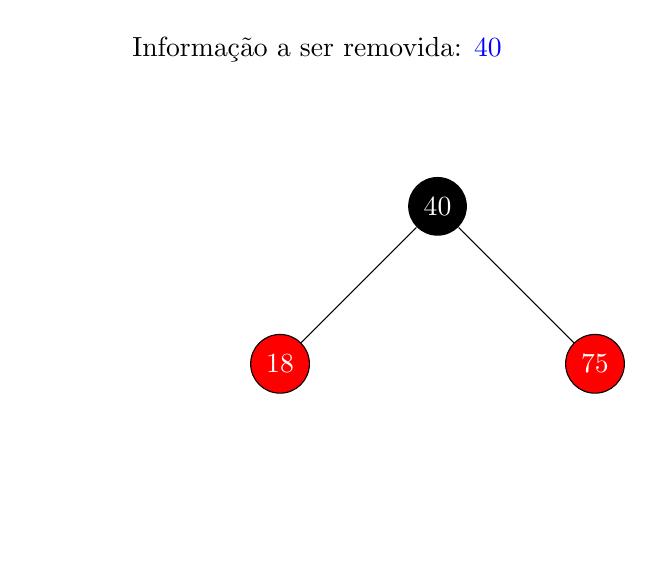
\begin{tikzpicture}
        \begin{scope}{shift={(3,0)}}
            \node[opacity=0] (X) at (-1, 2) { $1$ };
            \node[anchor=west] at (0, 8) { Informação a ser removida: \textcolor{blue}{40} };
            \node[circle,fill=black] (A) at (4, 6) { \textcolor{white}{40} };
            \node[circle,draw,fill=red] (B) at (2, 4) { \textcolor{white}{18} };
            \node[circle,draw,fill=red] (C) at (6, 4) { \textcolor{white}{75} };

            \draw (A) -- (B);
            \draw (A) -- (C);
        \end{scope}
    \end{tikzpicture}

\end{frame}

\begin{frame}[fragile]{Exemplo de remoção de nó vermelho}

    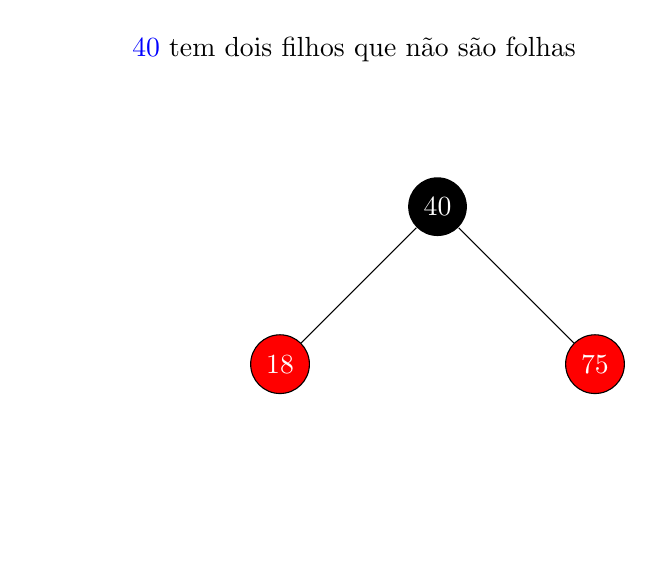
\begin{tikzpicture}
        \begin{scope}{shift={(3,0)}}
            \node[opacity=0] (X) at (-1, 2) { $1$ };
            \node[anchor=west] at (0, 8) { \textcolor{blue}{40} tem dois filhos que não são folhas };
            \node[circle,fill=black] (A) at (4, 6) { \textcolor{white}{40} };
            \node[circle,draw,fill=red] (B) at (2, 4) { \textcolor{white}{18} };
            \node[circle,draw,fill=red] (C) at (6, 4) { \textcolor{white}{75} };

            \draw (A) -- (B);
            \draw (A) -- (C);
        \end{scope}
    \end{tikzpicture}

\end{frame}

\begin{frame}[fragile]{Exemplo de remoção de nó vermelho}

    \begin{tikzpicture}
        \begin{scope}{shift={(3,0)}}
            \node[opacity=0] (X) at (-1, 2) { $1$ };
            \node[anchor=west] at (0, 8) { Redução ao caso 1 ou ao caso 2 };
            \draw[ultra thick,blue] (A) circle [radius=12pt];
            \node[circle,fill=black] (A) at (4, 6) { \textcolor{white}{40} };
            \node[circle,draw,fill=red] (B) at (2, 4) { \textcolor{white}{18} };
            \node[circle,draw,fill=red] (C) at (6, 4) { \textcolor{white}{75} };

            \draw (A) -- (B);
            \draw (A) -- (C);

        \end{scope}
    \end{tikzpicture}

\end{frame}

\begin{frame}[fragile]{Exemplo de remoção de nó vermelho}

    \begin{tikzpicture}
        \begin{scope}{shift={(3,0)}}
            \node[opacity=0] (X) at (-1, 2) { $1$ };
            \node[anchor=west] at (0, 8) { Redução ao caso 1 ou ao caso 2 };
            \draw[ultra thick,blue] (A) circle [radius=12pt];
            \node[circle,fill=black] (A) at (4, 6) { \textcolor{white}{40} };
            \draw[ultra thick,black!30!green] (B) circle [radius=12pt];
            \node[circle,draw,fill=red] (B) at (2, 4) { \textcolor{white}{18} };
            \node[circle,draw,fill=red] (C) at (6, 4) { \textcolor{white}{75} };

            \draw (A) -- (B);
            \draw (A) -- (C);

        \end{scope}
    \end{tikzpicture}

\end{frame}

\begin{frame}[fragile]{Exemplo de remoção de nó vermelho}

    \begin{tikzpicture}
        \begin{scope}{shift={(3,0)}}
            \node[opacity=0] (X) at (-1, 2) { $1$ };
            \node[anchor=west] at (0, 8) { Redução ao caso 1 ou ao caso 2 };
            \draw[ultra thick,blue] (B) circle [radius=12pt];
            \node[circle,fill=black] (A) at (4, 6) { \textcolor{white}{18} };
            \draw[ultra thick,black!30!green] (A) circle [radius=12pt];
            \node[circle,draw,fill=red] (B) at (2, 4) { \textcolor{white}{40} };
            \node[circle,draw,fill=red] (C) at (6, 4) { \textcolor{white}{75} };

            \draw (A) -- (B);
            \draw (A) -- (C);

        \end{scope}
    \end{tikzpicture}

\end{frame}

\begin{frame}[fragile]{Exemplo de remoção de nó vermelho}

    \begin{tikzpicture}
        \begin{scope}{shift={(3,0)}}
            \node[opacity=0] (X) at (-1, 2) { $1$ };
            \node[anchor=west] at (0, 8) { Remoção de nó vermelho sem filhos que não sejam folhas };
            \draw[ultra thick,blue] (B) circle [radius=12pt];
            \node[circle,fill=black] (A) at (4, 6) { \textcolor{white}{18} };
            \node[circle,draw,fill=red] (B) at (2, 4) { \textcolor{white}{40} };
            \node[circle,draw,fill=red] (C) at (6, 4) { \textcolor{white}{75} };

            \draw (A) -- (B);
            \draw (A) -- (C);

        \end{scope}
    \end{tikzpicture}

\end{frame}

\begin{frame}[fragile]{Exemplo de remoção de nó vermelho}

    \begin{tikzpicture}
        \begin{scope}{shift={(3,0)}}
            \node[opacity=0] (X) at (-1, 2) { $1$ };
            \node[anchor=west] at (0, 8) { Remoção de nó vermelho sem filhos que não sejam folhas };
            \draw[ultra thick,blue] (B) circle [radius=12pt];
            \node[circle,fill=black] (A) at (4, 6) { \textcolor{white}{18} };
            \node[circle,draw,fill=red] (B) at (2, 4) { \textcolor{white}{40} };
            \node[circle,draw,fill=red] (C) at (6, 4) { \textcolor{white}{75} };

            \draw (A) -- (C);

        \end{scope}
    \end{tikzpicture}

\end{frame}

\begin{frame}[fragile]{Exemplo de remoção de nó vermelho}

    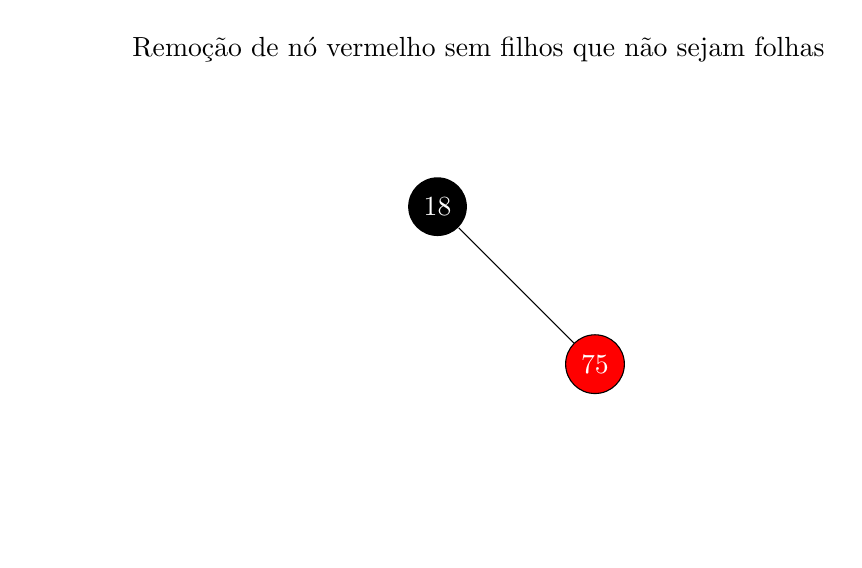
\begin{tikzpicture}
        \begin{scope}{shift={(3,0)}}
            \node[opacity=0] (X) at (-1, 2) { $1$ };
            \node[anchor=west] at (0, 8) { Remoção de nó vermelho sem filhos que não sejam folhas };
%            \draw[ultra thick,blue] (B) circle [radius=12pt];
            \node[circle,fill=black] (A) at (4, 6) { \textcolor{white}{18} };
%            \node[circle,draw,fill=red] (B) at (2, 4) { \textcolor{white}{40} };
            \node[circle,draw,fill=red] (C) at (6, 4) { \textcolor{white}{75} };

            \draw (A) -- (C);

        \end{scope}
    \end{tikzpicture}

\end{frame}

\begin{frame}[fragile]{Implementação da remoção de nó vermelho}
    \inputsnippet{cpp}{194}{207}{rb.cpp}
\end{frame}

\begin{frame}[fragile]{Remoção de nó preto com filho vermelho}

    \begin{itemize}
        \item Se $N$ é preto e seu filho $C$ é vermelho, a remoção de $N$ viola a propriedade 5,
            devido a redução no número de nós pretos

        \item Além disso, a promoção de um nó vermelho pode levar a violação da propriedade 4

        \item Uma forma de preservar ambas propriedades é recolorir $C$ como um nó preto

        \item Isto restaura a violação da propriedade 5, pois a perda de $N$ agora é compensada
            com a adição de um novo nó preto

        \item O fato de $C$ assumir a cor preta evita que a propriedade 4 seja violada
    \end{itemize}

\end{frame}

\begin{frame}[fragile]{Exemplo de remoção de nó vermelho}

    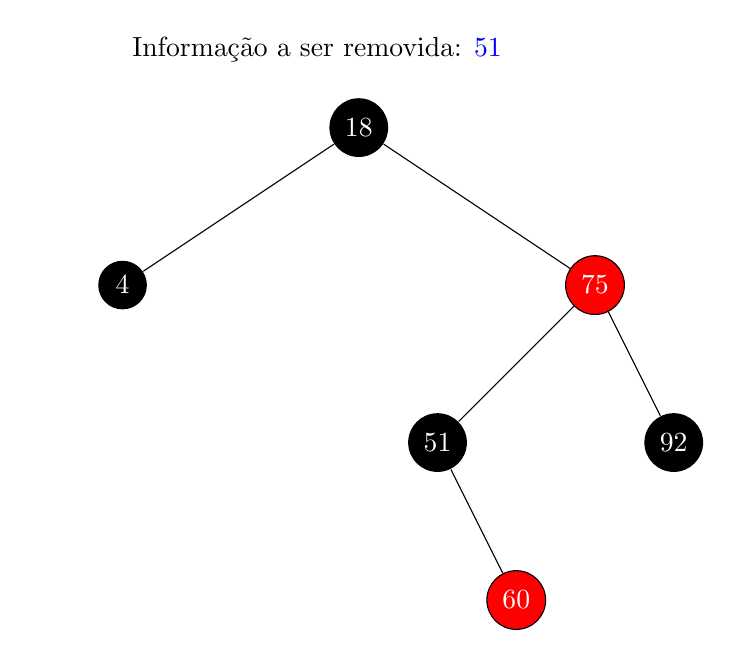
\begin{tikzpicture}
        \begin{scope}{shift={(3,0)}}
            \node[opacity=0] (X) at (-1, 2) { $1$ };
            \node[anchor=west] at (0, 8) { Informação a ser removida: \textcolor{blue}{51} };
%            \draw[ultra thick,blue] (B) circle [radius=12pt];
            \node[circle,fill=black] (A) at (3, 7) { \textcolor{white}{18} };
            \node[circle,fill=black] (B) at (0, 5) { \textcolor{white}{4} };
            \node[circle,draw,fill=red] (C) at (6, 5) { \textcolor{white}{75} };
            \node[circle,fill=black] (D) at (4, 3) { \textcolor{white}{51} };
            \node[circle,fill=black] (E) at (7, 3) { \textcolor{white}{92} };
            \node[circle,draw,fill=red] (F) at (5, 1) { \textcolor{white}{60} };

            \draw (A) -- (B);
            \draw (A) -- (C);
            \draw (C) -- (D);
            \draw (C) -- (E);
            \draw (D) -- (F);

        \end{scope}
    \end{tikzpicture}

\end{frame}

\begin{frame}[fragile]{Exemplo de remoção de nó vermelho}

    \begin{tikzpicture}
        \begin{scope}{shift={(3,0)}}
            \node[opacity=0] (X) at (-1, 2) { $1$ };
            \node[anchor=west] at (0, 8) { Informação a ser removida: \textcolor{blue}{51} };
            \draw[ultra thick,blue] (A) circle [radius=12pt];
            \node[circle,fill=black] (A) at (3, 7) { \textcolor{white}{18} };
            \node[circle,fill=black] (B) at (0, 5) { \textcolor{white}{4} };
            \node[circle,draw,fill=red] (C) at (6, 5) { \textcolor{white}{75} };
            \node[circle,fill=black] (D) at (4, 3) { \textcolor{white}{51} };
            \node[circle,fill=black] (E) at (7, 3) { \textcolor{white}{92} };
            \node[circle,draw,fill=red] (F) at (5, 1) { \textcolor{white}{60} };

            \draw (A) -- (B);
            \draw (A) -- (C);
            \draw (C) -- (D);
            \draw (C) -- (E);
            \draw (D) -- (F);

        \end{scope}
    \end{tikzpicture}

\end{frame}

\begin{frame}[fragile]{Exemplo de remoção de nó vermelho}

    \begin{tikzpicture}
        \begin{scope}{shift={(3,0)}}
            \node[opacity=0] (X) at (-1, 2) { $1$ };
            \node[anchor=west] at (0, 8) { Informação a ser removida: \textcolor{blue}{51} };
            \draw[ultra thick,blue] (C) circle [radius=12pt];
            \node[circle,fill=black] (A) at (3, 7) { \textcolor{white}{18} };
            \node[circle,fill=black] (B) at (0, 5) { \textcolor{white}{4} };
            \node[circle,draw,fill=red] (C) at (6, 5) { \textcolor{white}{75} };
            \node[circle,fill=black] (D) at (4, 3) { \textcolor{white}{51} };
            \node[circle,fill=black] (E) at (7, 3) { \textcolor{white}{92} };
            \node[circle,draw,fill=red] (F) at (5, 1) { \textcolor{white}{60} };

            \draw (A) -- (B);
            \draw (A) -- (C);
            \draw (C) -- (D);
            \draw (C) -- (E);
            \draw (D) -- (F);

        \end{scope}
    \end{tikzpicture}

\end{frame}

\begin{frame}[fragile]{Exemplo de remoção de nó vermelho}

    \begin{tikzpicture}
        \begin{scope}{shift={(3,0)}}
            \node[opacity=0] (X) at (-1, 2) { $1$ };
            \node[anchor=west] at (0, 8) { Informação a ser removida: \textcolor{blue}{51} };
            \draw[ultra thick,blue] (D) circle [radius=12pt];
            \node[circle,fill=black] (A) at (3, 7) { \textcolor{white}{18} };
            \node[circle,fill=black] (B) at (0, 5) { \textcolor{white}{4} };
            \node[circle,draw,fill=red] (C) at (6, 5) { \textcolor{white}{75} };
            \node[circle,fill=black] (D) at (4, 3) { \textcolor{white}{51} };
            \node[circle,fill=black] (E) at (7, 3) { \textcolor{white}{92} };
            \node[circle,draw,fill=red] (F) at (5, 1) { \textcolor{white}{60} };

            \draw (A) -- (B);
            \draw (A) -- (C);
            \draw (C) -- (D);
            \draw (C) -- (E);
            \draw (D) -- (F);

        \end{scope}
    \end{tikzpicture}

\end{frame}

\begin{frame}[fragile]{Exemplo de remoção de nó vermelho}

    \begin{tikzpicture}
        \begin{scope}{shift={(3,0)}}
            \node[opacity=0] (X) at (-1, 2) { $1$ };
            \node[anchor=west] at (0, 8) { Nó preto com filho vermelho };
            \draw[ultra thick,blue] (D) circle [radius=12pt];
            \draw[ultra thick,black!30!green] (F) circle [radius=12pt];
            \node[circle,fill=black] (A) at (3, 7) { \textcolor{white}{18} };
            \node[circle,fill=black] (B) at (0, 5) { \textcolor{white}{4} };
            \node[circle,draw,fill=red] (C) at (6, 5) { \textcolor{white}{75} };
            \node[circle,fill=black] (D) at (4, 3) { \textcolor{white}{51} };
            \node[circle,fill=black] (E) at (7, 3) { \textcolor{white}{92} };
            \node[circle,draw,fill=red] (F) at (5, 1) { \textcolor{white}{60} };

            \draw (A) -- (B);
            \draw (A) -- (C);
            \draw (C) -- (D);
            \draw (C) -- (E);
            \draw (D) -- (F);

        \end{scope}
    \end{tikzpicture}

\end{frame}

\begin{frame}[fragile]{Exemplo de remoção de nó vermelho}

    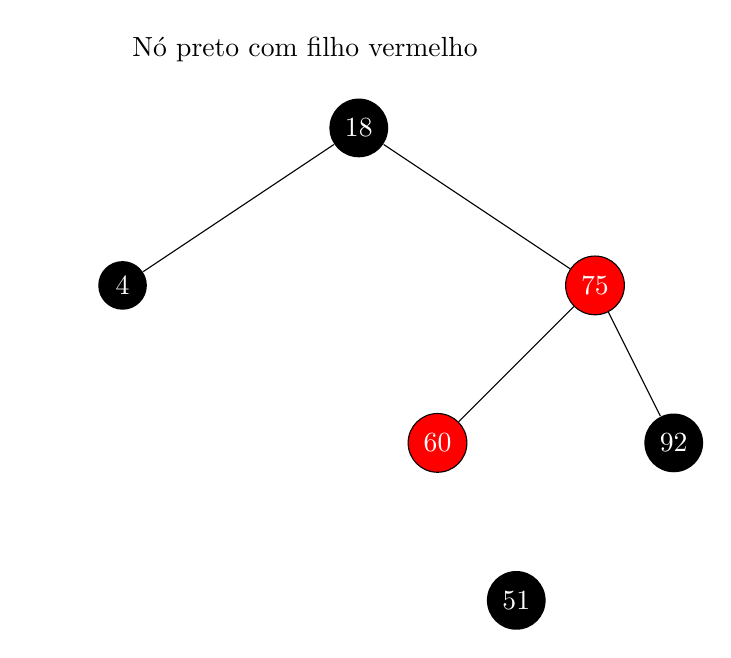
\begin{tikzpicture}
        \begin{scope}{shift={(3,0)}}
            \node[opacity=0] (X) at (-1, 2) { $1$ };
            \node[anchor=west] at (0, 8) { Nó preto com filho vermelho };
%            \draw[ultra thick,blue] (D) circle [radius=12pt];
%            \draw[ultra thick,black!30!green] (F) circle [radius=12pt];
            \node[circle,fill=black] (A) at (3, 7) { \textcolor{white}{18} };
            \node[circle,fill=black] (B) at (0, 5) { \textcolor{white}{4} };
            \node[circle,draw,fill=red] (C) at (6, 5) { \textcolor{white}{75} };
            \node[circle,fill=black] (D) at (5, 1) { \textcolor{white}{51} };
            \node[circle,fill=black] (E) at (7, 3) { \textcolor{white}{92} };
            \node[circle,draw,fill=red] (F) at (4, 3) { \textcolor{white}{60} };

            \draw (A) -- (B);
            \draw (A) -- (C);
            \draw (C) -- (E);
            \draw (C) -- (F);

        \end{scope}
    \end{tikzpicture}

\end{frame}

\begin{frame}[fragile]{Exemplo de remoção de nó vermelho}

    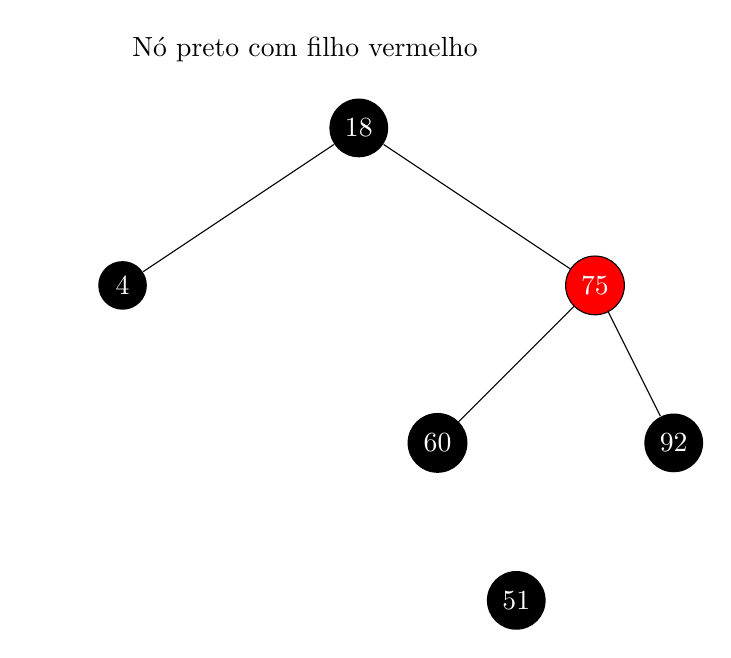
\begin{tikzpicture}
        \begin{scope}{shift={(3,0)}}
            \node[opacity=0] (X) at (-1, 2) { $1$ };
            \node[anchor=west] at (0, 8) { Nó preto com filho vermelho };
%            \draw[ultra thick,blue] (D) circle [radius=12pt];
%            \draw[ultra thick,black!30!green] (F) circle [radius=12pt];
            \node[circle,fill=black] (A) at (3, 7) { \textcolor{white}{18} };
            \node[circle,fill=black] (B) at (0, 5) { \textcolor{white}{4} };
            \node[circle,draw,fill=red] (C) at (6, 5) { \textcolor{white}{75} };
            \node[circle,fill=black] (D) at (5, 1) { \textcolor{white}{51} };
            \node[circle,fill=black] (E) at (7, 3) { \textcolor{white}{92} };
            \node[circle,draw,fill=black] (F) at (4, 3) { \textcolor{white}{60} };

            \draw (A) -- (B);
            \draw (A) -- (C);
            \draw (C) -- (E);
            \draw (C) -- (F);

        \end{scope}
    \end{tikzpicture}

\end{frame}

\begin{frame}[fragile]{Exemplo de remoção de nó vermelho}

    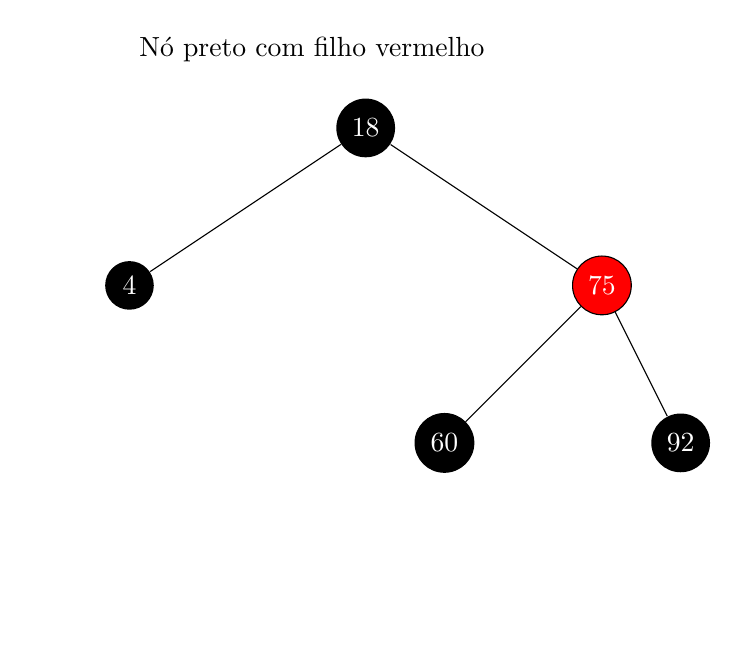
\begin{tikzpicture}
        \begin{scope}{shift={(3,0)}}
            \node[opacity=0] (X) at (-1, 1) { $51$ };
            \node[anchor=west] at (0, 8) { Nó preto com filho vermelho };
%            \draw[ultra thick,blue] (D) circle [radius=12pt];
%            \draw[ultra thick,black!30!green] (F) circle [radius=12pt];
            \node[circle,fill=black] (A) at (3, 7) { \textcolor{white}{18} };
            \node[circle,fill=black] (B) at (0, 5) { \textcolor{white}{4} };
            \node[circle,draw,fill=red] (C) at (6, 5) { \textcolor{white}{75} };
%            \node[circle,fill=black] (D) at (5, 1) { \textcolor{white}{51} };
            \node[circle,fill=black] (E) at (7, 3) { \textcolor{white}{92} };
            \node[circle,draw,fill=black] (F) at (4, 3) { \textcolor{white}{60} };

            \draw (A) -- (B);
            \draw (A) -- (C);
            \draw (C) -- (E);
            \draw (C) -- (F);

        \end{scope}
    \end{tikzpicture}

\end{frame}

\begin{frame}[fragile]{Implementação da remoção de nó preto com filho vermelho}
    \inputsnippet{cpp}{208}{215}{rb.cpp}
\end{frame}

\begin{frame}[fragile]{Nó preto com filho preto}

    \begin{itemize}
        \item O caso onde ambos $N$ e $C$ são pretos é o mais complexo dentre todos os que
            envolvem um nó com, no máximo, um filho não-folha

        \item A remoção de um nó preto viola a propriedade 5 das árvores \textit{red-black}

        \item Há múltiplos cenários possíveis, cada um tendo que ser tratado adequadamente

        \item Observe que este caso ocorre apenas quando ambos filhos de $N$ são folhas

        \item Isto porque se $N$ tivesse apenas uma folha preta, o fato do outro filho não ser
            folha violaria a propriedade 5
    \end{itemize}

\end{frame}

\begin{frame}[fragile]{Cenário A: após a troca de $N$ e $C$, $C$ é raiz}

    \begin{itemize}
        \item Este é o cenário mais simples

        \item A remoção de um nó preto da posição raiz subtrai igualmente uma unidade de todos
            os caminhos da raiz às folhas

        \item Assim a propriedade 5 fica preservada

        \item As demais propriedades também se mantém: como as folhas são pretas, a raiz também
            será preta
    \end{itemize}

    \inputsnippet{cpp}{216}{222}{rb.cpp}
\end{frame}

\begin{frame}[fragile]{Exemplo de remoção no cenário A}

    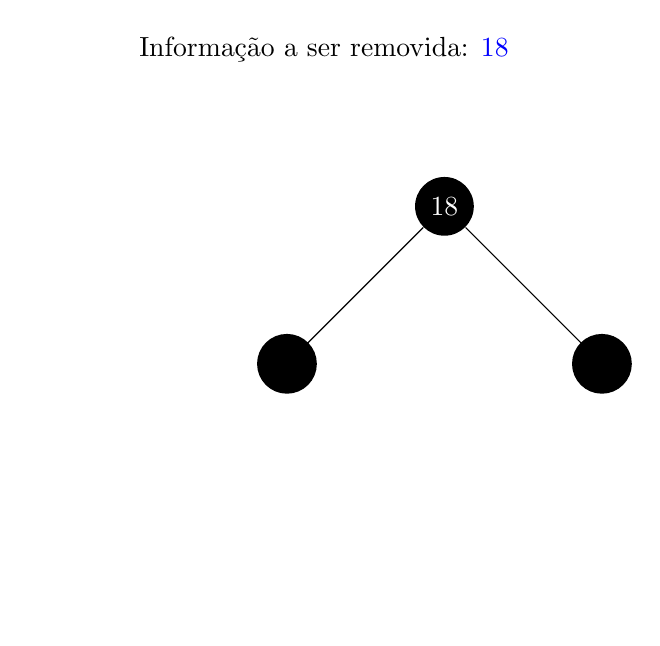
\begin{tikzpicture}
        \begin{scope}{shift={(3,0)}}
            \node[opacity=0] (X) at (-1, 1) { $51$ };
            \node[anchor=west] at (0, 8) { Informação a ser removida: \textcolor{blue}{18} };
            \node[opacity=0] (B) at (2, 4) { };
            \node[opacity=0] (C) at (6, 4) { };

            \draw[ultra thick,fill=black] (B) circle [radius=10pt];
            \draw[ultra thick,fill=black] (C) circle [radius=10pt];
            \node[circle,fill=black] (A) at (4, 6) { \textcolor{white}{18} };

            \draw (A) -- (B);
            \draw (A) -- (C);

        \end{scope}
    \end{tikzpicture}

\end{frame}

\begin{frame}[fragile]{Exemplo de remoção no cenário A}

    \begin{tikzpicture}
        \begin{scope}{shift={(3,0)}}
            \node[opacity=0] (X) at (-1, 1) { $51$ };
            \node[anchor=west] at (0, 8) { Informação a ser removida: \textcolor{blue}{18} };
            \node[opacity=0] (B) at (2, 4) { };
            \node[opacity=0] (C) at (6, 4) { };

            \draw[ultra thick,blue] (A) circle [radius=12pt];
            \draw[ultra thick,fill=black] (B) circle [radius=10pt];
            \draw[ultra thick,fill=black] (C) circle [radius=10pt];
            \node[circle,fill=black] (A) at (4, 6) { \textcolor{white}{18} };

            \draw (A) -- (B);
            \draw (A) -- (C);

        \end{scope}
    \end{tikzpicture}

\end{frame}

\begin{frame}[fragile]{Exemplo de remoção no cenário A}

    \begin{tikzpicture}
        \begin{scope}{shift={(3,0)}}
            \node[opacity=0] (X) at (-1, 1) { $51$ };
            \node[anchor=west] at (0, 8) { Informação a ser removida: \textcolor{blue}{18} };
            \node[opacity=0] (B) at (2, 4) { };
            \node[opacity=0] (C) at (6, 4) { };

            \draw[ultra thick,blue] (A) circle [radius=12pt];
            \draw[ultra thick,fill=black] (B) circle [radius=10pt];
            \draw[ultra thick,black!30!green] (B) circle [radius=12pt];
            \draw[ultra thick,fill=black] (C) circle [radius=10pt];
            \node[circle,fill=black] (A) at (4, 6) { \textcolor{white}{18} };

            \draw (A) -- (B);
            \draw (A) -- (C);

        \end{scope}
    \end{tikzpicture}

\end{frame}

\begin{frame}[fragile]{Exemplo de remoção no cenário A}

    \begin{tikzpicture}
        \begin{scope}{shift={(3,0)}}
            \node[opacity=0] (X) at (-1, 1) { $51$ };
            \node[anchor=west] at (0, 8) { Informação a ser removida: \textcolor{blue}{18} };
            \node[opacity=0] (A) at (4, 6) { };
            \node[opacity=0] (C) at (6, 4) { };

            \draw[ultra thick,blue] (B) circle [radius=12pt];
            \draw[ultra thick,fill=black] (A) circle [radius=10pt];
            \draw[ultra thick,black!30!green] (A) circle [radius=12pt];
            \draw[ultra thick,fill=black] (C) circle [radius=10pt];
            \node[circle,fill=black] (B) at (2, 4) { \textcolor{white}{18} };

        \end{scope}
    \end{tikzpicture}

\end{frame}

\begin{frame}[fragile]{Exemplo de remoção no cenário A}

    \begin{tikzpicture}
        \begin{scope}{shift={(3,0)}}
            \node[opacity=0] (X) at (-1, 1) { $51$ };
            \node[anchor=west] at (0, 8) { Informação a ser removida: \textcolor{blue}{18} };
%            \node[opacity=0] (A) at (4, 6) { };
%            \node[opacity=0] (C) at (6, 4) { };

%            \draw[ultra thick,blue] (B) circle [radius=12pt];
            \draw[ultra thick,fill=black] (A) circle [radius=10pt];
%            \draw[ultra thick,black!30!green] (A) circle [radius=12pt];
%            \draw[ultra thick,fill=black] (C) circle [radius=10pt];
%            \node[circle,fill=black] (B) at (2, 4) { \textcolor{white}{18} };

        \end{scope}
    \end{tikzpicture}

\end{frame}

\begin{frame}[fragile]{Cenário B: Irmão vermelho}

    \begin{itemize}
        \item Se o nó a ser removido tem um irmão $S$ vermelho, é preciso promover um 
            reposicionamento dos nós, além de uma troca de cores entre o pai $P$ e o irmão $S$

        \item Este cenário não pode ser resolvido diretamente: o resultado deste reposicionamento
            levará a um dos próximos cenários

        \item Primeiramente as cores de $P$ e $S$ devem ser trocadas

        \item Uma rotação de $S$ em torno de $P$, o torna o novo avô de $N$

        \item Ao final deste processo uma das duas subárvores terá caminho da raiz até uma folha
            uma unidade menor do que a outra, violando a propriedade 5

        \item Porém o caso a ser tratado mudou: agora $N$ tem pai vermelho, com irmão preto

        \item Este cenário será abordado mais adiante
    \end{itemize}

\end{frame}

\begin{frame}[fragile]{Exemplo de remoção no cenário B}

    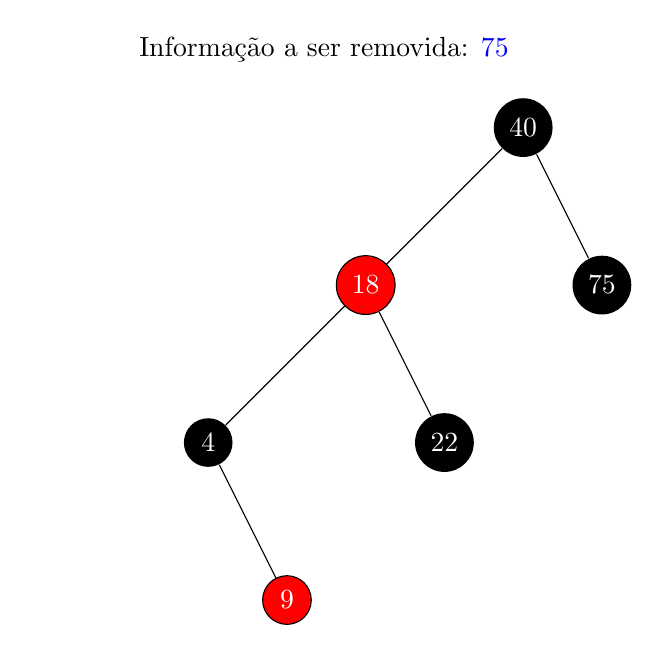
\begin{tikzpicture}
        \begin{scope}{shift={(3,0)}}
            \node[opacity=0] (X) at (-1, 1) { $51$ };
            \node[anchor=west] at (0, 8) { Informação a ser removida: \textcolor{blue}{75} };
%            \draw[ultra thick,fill=black] (A) circle [radius=10pt];
            \node[circle,fill=black] (A) at (5, 7) { \textcolor{white}{40} };
            \node[circle,draw,fill=red] (B) at (3, 5) { \textcolor{white}{18} };
            \node[circle,fill=black] (C) at (6, 5) { \textcolor{white}{75} };
            \node[circle,fill=black] (D) at (1, 3) { \textcolor{white}{4} };
            \node[circle,fill=black] (E) at (4, 3) { \textcolor{white}{22} };
            \node[circle,draw,fill=red] (F) at (2, 1) { \textcolor{white}{9} };

            \draw (A) -- (B);
            \draw (A) -- (C);
            \draw (B) -- (D);
            \draw (B) -- (E);
            \draw (D) -- (F);

        \end{scope}
    \end{tikzpicture}

\end{frame}

\begin{frame}[fragile]{Exemplo de remoção no cenário B}

    \begin{tikzpicture}
        \begin{scope}{shift={(3,0)}}
            \node[opacity=0] (X) at (-1, 1) { $51$ };
            \node[anchor=west] at (0, 8) { Informação a ser removida: \textcolor{blue}{75} };
            \draw[ultra thick,blue] (A) circle [radius=12pt];
            \node[circle,fill=black] (A) at (5, 7) { \textcolor{white}{40} };
            \node[circle,draw,fill=red] (B) at (3, 5) { \textcolor{white}{18} };
            \node[circle,fill=black] (C) at (6, 5) { \textcolor{white}{75} };
            \node[circle,fill=black] (D) at (1, 3) { \textcolor{white}{4} };
            \node[circle,fill=black] (E) at (4, 3) { \textcolor{white}{22} };
            \node[circle,draw,fill=red] (F) at (2, 1) { \textcolor{white}{9} };

            \draw (A) -- (B);
            \draw (A) -- (C);
            \draw (B) -- (D);
            \draw (B) -- (E);
            \draw (D) -- (F);

        \end{scope}
    \end{tikzpicture}

\end{frame}

\begin{frame}[fragile]{Exemplo de remoção no cenário B}

    \begin{tikzpicture}
        \begin{scope}{shift={(3,0)}}
            \node[opacity=0] (X) at (-1, 1) { $51$ };
            \node[anchor=west] at (0, 8) { Informação a ser removida: \textcolor{blue}{75} };
            \draw[ultra thick,blue] (C) circle [radius=12pt];
            \node[circle,fill=black] (A) at (5, 7) { \textcolor{white}{40} };
            \node[circle,draw,fill=red] (B) at (3, 5) { \textcolor{white}{18} };
            \node[circle,fill=black] (C) at (6, 5) { \textcolor{white}{75} };
            \node[circle,fill=black] (D) at (1, 3) { \textcolor{white}{4} };
            \node[circle,fill=black] (E) at (4, 3) { \textcolor{white}{22} };
            \node[circle,draw,fill=red] (F) at (2, 1) { \textcolor{white}{9} };

            \draw (A) -- (B);
            \draw (A) -- (C);
            \draw (B) -- (D);
            \draw (B) -- (E);
            \draw (D) -- (F);

        \end{scope}
    \end{tikzpicture}

\end{frame}

\begin{frame}[fragile]{Exemplo de remoção no cenário B}

    \begin{tikzpicture}
        \begin{scope}{shift={(3,0)}}
            \node[opacity=0] (X) at (-1, 1) { $51$ };
            \node[anchor=west] at (0, 8) { Informação a ser removida: \textcolor{black}{75} };
            \draw[ultra thick,fill=black] (C) circle [radius=10pt];
            \node[circle,fill=black] (A) at (5, 7) { \textcolor{white}{40} };
            \node[circle,draw,fill=red] (B) at (3, 5) { \textcolor{white}{18} };
%            \node[circle,fill=black] (C) at (6, 5) { \textcolor{white}{75} };
            \node[circle,fill=black] (D) at (1, 3) { \textcolor{white}{4} };
            \node[circle,fill=black] (E) at (4, 3) { \textcolor{white}{22} };
            \node[circle,draw,fill=red] (F) at (2, 1) { \textcolor{white}{9} };

            \draw (A) -- (B);
            \draw (A) -- (C);
            \draw (B) -- (D);
            \draw (B) -- (E);
            \draw (D) -- (F);

        \end{scope}
    \end{tikzpicture}

\end{frame}

\begin{frame}[fragile]{Exemplo de remoção no cenário B}

    \begin{tikzpicture}
        \begin{scope}{shift={(3,0)}}
            \node[opacity=0] (X) at (-1, 1) { $51$ };
            \node[anchor=west] at (0, 8) { Nó preto, irmão vermelho };
            \draw[ultra thick,fill=black] (C) circle [radius=10pt];
            \draw[ultra thick,blue] (C) circle [radius=12pt];
            \draw[ultra thick,black!30!green] (B) circle [radius=12pt];
            \node[circle,fill=black] (A) at (5, 7) { \textcolor{white}{40} };
            \node[circle,draw,fill=red] (B) at (3, 5) { \textcolor{white}{18} };
%            \node[circle,fill=black] (C) at (6, 5) { \textcolor{white}{75} };
            \node[circle,fill=black] (D) at (1, 3) { \textcolor{white}{4} };
            \node[circle,fill=black] (E) at (4, 3) { \textcolor{white}{22} };
            \node[circle,draw,fill=red] (F) at (2, 1) { \textcolor{white}{9} };

            \draw (A) -- (B);
            \draw (A) -- (C);
            \draw (B) -- (D);
            \draw (B) -- (E);
            \draw (D) -- (F);

        \end{scope}
    \end{tikzpicture}

\end{frame}

\begin{frame}[fragile]{Exemplo de remoção no cenário B}

    \begin{tikzpicture}
        \begin{scope}{shift={(3,0)}}
            \node[opacity=0] (X) at (-1, 1) { $51$ };
            \node[anchor=west] at (0, 8) { Nó preto, irmão vermelho };
            \draw[ultra thick,fill=black] (C) circle [radius=10pt];
            \draw[ultra thick,blue] (C) circle [radius=12pt];
            \draw[ultra thick,black!30!green] (B) circle [radius=12pt];
            \node[circle,draw,fill=red] (A) at (5, 7) { \textcolor{white}{40} };
            \node[circle,draw,fill=black] (B) at (3, 5) { \textcolor{white}{18} };
%            \node[circle,fill=black] (C) at (6, 5) { \textcolor{white}{75} };
            \node[circle,fill=black] (D) at (1, 3) { \textcolor{white}{4} };
            \node[circle,fill=black] (E) at (4, 3) { \textcolor{white}{22} };
            \node[circle,draw,fill=red] (F) at (2, 1) { \textcolor{white}{9} };

            \draw (A) -- (B);
            \draw (A) -- (C);
            \draw (B) -- (D);
            \draw (B) -- (E);
            \draw (D) -- (F);

        \end{scope}
    \end{tikzpicture}

\end{frame}

\begin{frame}[fragile]{Exemplo de remoção no cenário B}

    \begin{tikzpicture}
        \begin{scope}{shift={(3,0)}}
            \node[opacity=0] (X) at (-1, 1) { $51$ };
            \node[opacity=0] (G) at (7, 3) { $51$ };
            \node[anchor=west] at (0, 8) { Nó preto, irmão vermelho };
            \draw[ultra thick,fill=black] (C) circle [radius=10pt];
            \draw[ultra thick,blue] (G) circle [radius=12pt];
            \draw[ultra thick,fill=black] (G) circle [radius=10pt];
            \node[circle,draw,fill=red] (A) at (6, 5) { \textcolor{white}{40} };
            \node[circle,draw,fill=black] (B) at (4, 7) { \textcolor{white}{18} };
            \draw[ultra thick,black!30!green] (B) circle [radius=12pt];
            \node[circle,fill=black] (D) at (2, 5) { \textcolor{white}{4} };
            \node[circle,fill=black] (E) at (5, 3) { \textcolor{white}{22} };
            \node[circle,draw,fill=red] (F) at (3, 3) { \textcolor{white}{9} };

            \draw (A) -- (B);
            \draw (A) -- (C);
            \draw (B) -- (D);
            \draw (A) -- (E);
            \draw (D) -- (F);
            \draw (A) -- (G);

        \end{scope}
    \end{tikzpicture}

\end{frame}

\begin{frame}[fragile]{Implementação do cenário B}
    \inputsnippet{cpp}{222}{240}{rb.cpp}
\end{frame}


\begin{frame}[fragile]{Cenário C: 

    \begin{itemize}
        \item
    \end{itemize}

\end{frame}
